\chapter{Kafka and Spark}

\section{Introduction: scaling stream ingestion and processing}

To process a high volume of data, we need systems that are horizontally scalable. This means 
that we can add more machines to the system to increase its capacity. In this chapter, we will 
discuss two such systems: Apache Kafka and Apache Spark, and how they can be used together to
process large volumes of data.\\

In general, the roles of Kafka and Spark are as follows:

\begin{itemize}
    \item Kafka is used to collect and store data in real-time. It manages
    the ingestion of data from multiple sources and stores it in a distributed manner,
    making it available for processing by other systems.

    \item Spark is used to process the data stored in Kafka, and generate insights.
    It is a distributed computing system that can process large volumes of data in parallel.
\end{itemize}

Before getting into the details of Kafka and Spark, let's discuss some important concepts
that are used in these systems:

\begin{itemize}
    \item Latency vs throughput
    \item Data/message
\end{itemize}

\subsection{Latency vs throughput}

We refer to latency as the time taken for a message to travel from the producer to the consumer.
More generally, latency is the amount of time needed to complete a task. Throughput, on the other 
hand, is the number of messages that can be processed in a given time period.\\

We can see this with a visual example: consider a highway with cars moving at different speeds.
The latency is the time taken for a car to travel from one end of the highway to the other, while
the throughput is the number of cars that can pass through the highway in a certain time period,
say an hour.

\begin{figure}[H]
    \centering
    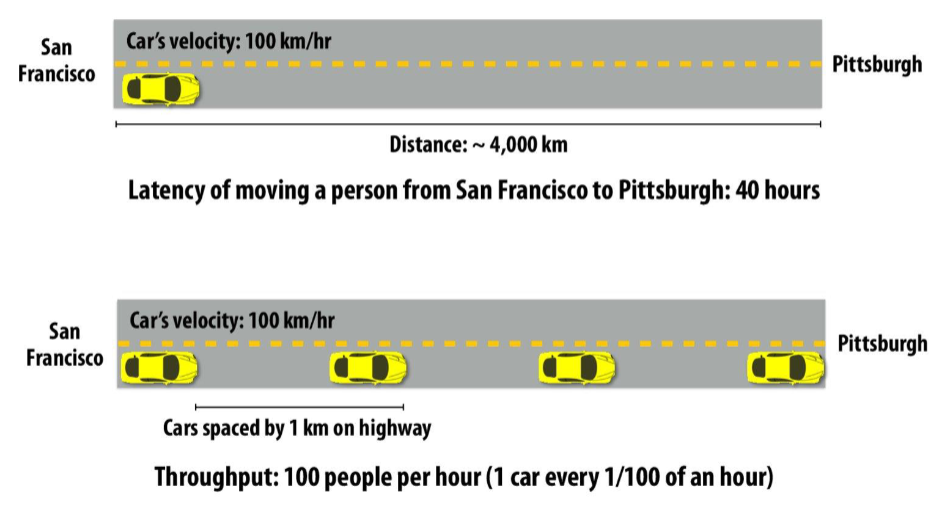
\includegraphics[width=0.6\textwidth]{figures/lat_vs_throu.png}
    \label{fig:latency_throughput}
    \caption{Latency vs throughput}
\end{figure}

We could improve the throughput by adding more lanes to the highway, but this would not necessarily
reduce the latency. To improve the latency, we would need to reduce the distance between the two ends
of the highway, or increase the speed of the cars. Notice that the latter would also improve the throughput,
as more cars would be able to pass through the highway in a given time period.

\begin{figure}[H]
    \centering
    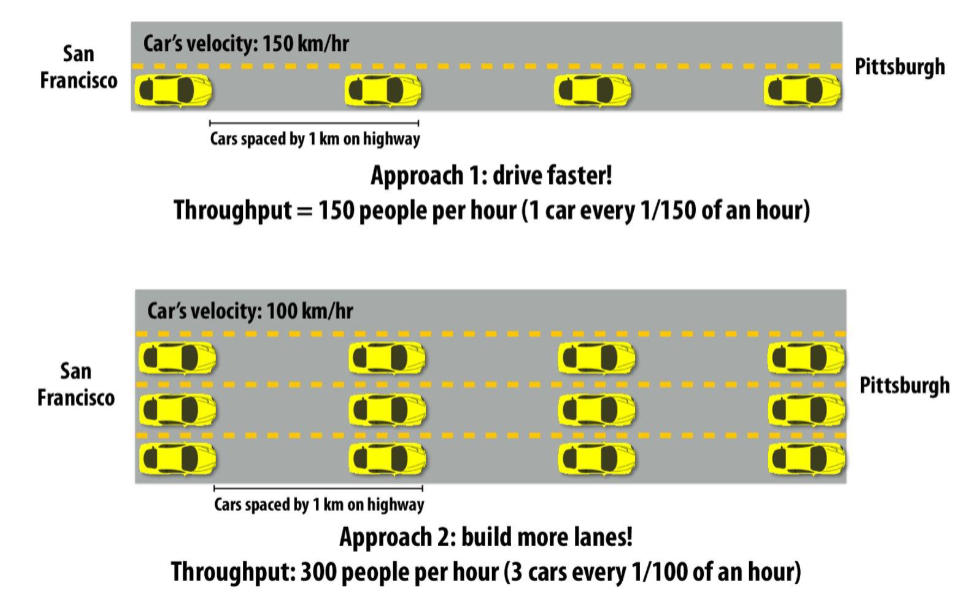
\includegraphics[width=0.6\textwidth]{figures/lat_vs_throu2.png}
    \label{fig:latency_throughput2}
    \caption{Improving latency and throughput}
\end{figure}

In the context of data processing, we usually want to minimize the latency and maximize the throughput.
This is because we want to process data as quickly as possible, and we want to be able to process a large
volume of data in a given time period.

\subsection{Data/message}

In the context of data processing, the data that comes in is usually in the form of messages. A message
is a unit of data that is sent from a producer to a consumer. For example, in a messaging system like Kafka,
a message could be a log entry, a sensor reading, or a user event. Messages can be of different types and sizes,
and can contain different types of data. For example, a message could be a JSON object, a binary blob, or a string.\\

Note that the way messages are represented can have a big impact on the performance of the system. Following the 
previous example, imagine that the messages are cars on a highway, and the people in the cars are the data. If the cars
are small and can carry only one person, then we would need a lot of cars to transport a large number of people. On the
other hand, if the cars are large and can carry many people, then we would need fewer cars to transport the same number
of people. The same is true for messages: if the messages are small, then we would need more of them to transport the same
amount of data, which would increase the overhead of the system. On the other hand, if the messages are large, then we would
need fewer of them to transport the same amount of data, which would reduce the overhead of the system.\\

In general, the larger the data poonts per message, the higher the throughput, but the higher the latency. This is because
larger messages take longer to process, but fewer of them are needed to transport the same amount of data.
So, it is needed to find a balance between the size of the messages and the performance of the system.\\

Compression and binary encodig are the typical ways to increase the data per message, given a fixed message size.

\section{Apache Kafka}

Apache Kafka is a distributed streaming platform that is used for building real-time data 
pipelines and streaming applications. It is designed to be scalable, fault-tolerant, and
highly available. Kafka is used for collecting, storing, and processing large volumes of data
in real-time. It is used by many companies, including LinkedIn, Netflix, Uber, and Airbnb, to
process data at scale.

\subsection{Kafka: high-level vs system view}

Let us take a conceptual view of Kafka. In general, Kafka is composed of the following components:

\begin{itemize}
    \item \textbf{Producer}: A producer is a system that sends data to Kafka. It sends the messages
    based on a certain topic.

    \item \textbf{Consumer}: A consumer is a system that reads data from Kafka. It consumes the messages
    from certain topics that subscribes to.

    \item \textbf{Topics}: A topic is a category of messages in Kafka. It is a way to organize the messages
    in Kafka. Producers send messages to topics, and consumers read messages from topics.

    \item \textbf{Messages}: A message is a unit of data in Kafka. It is a key-value pair that is sent 
    from a producer to a consumer. Messages are stored in topics and can be read by consumers.

    \item \textbf{Cluster}: A Kafka cluster manages a set of topics. 
\end{itemize}

\begin{figure}[H]
    \centering
    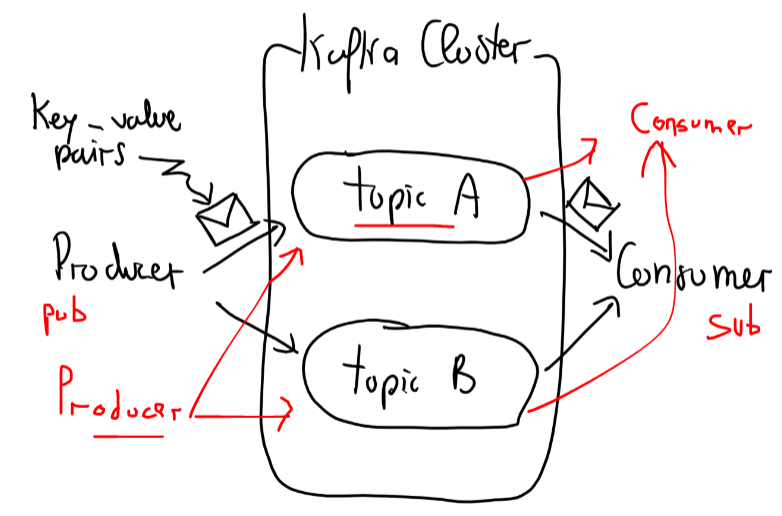
\includegraphics[width=0.4\textwidth]{figures/kafka_high_lev.png}
    \label{fig:kafka_high_lev}
    \caption{Kafka high-level view}
\end{figure}

This is a high-level view of Kafka. In practice, Kafka uses a distributed architecture to achieve
scalability, fault-tolerance, and high availability. So, for that, we need to introduce the
following concepts:

\begin{itemize}
    \item \textbf{Brokers}: A broker is a Kafka server that stores the messages. A Kafka cluster is composed
    of multiple brokers. Each broker stores a subset of the messages in the cluster.

    \item \textbf{Partitions}: A partition is a unit of parallelism in Kafka. A topic is divided into multiple
    partitions, and each partition is stored on a different broker. This allows Kafka to scale out by distributing
    the load across multiple brokers.
\end{itemize}

In general, a broker receives messages from producers, stores them in partitions, and serves them to consumers.
A production Kafka cluster typically consists of multiple brokers, each storing multiple partitions of multiple topics.
Each broker can handle a certain amount of traffic, and the cluster as a whole can handle a large volume
of data.\\

To ensure fault-tolerance, Kafka uses replication. Each partition is replicated across multiple brokers, so that
if one broker fails, the data is still available on other brokers. This allows Kafka to provide high availability
and durability.

\begin{figure}[H]
    \centering
    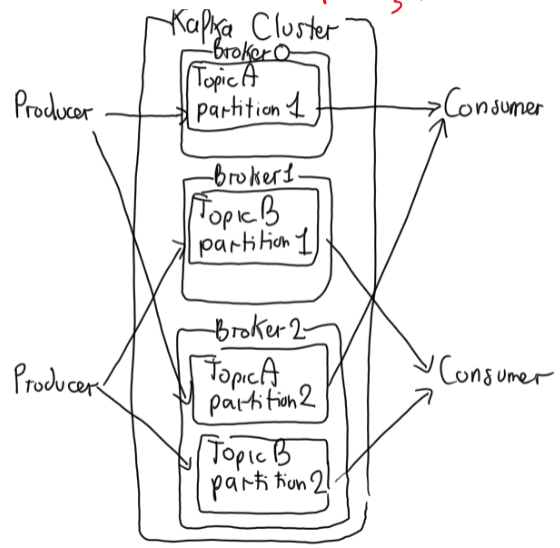
\includegraphics[width=0.35\textwidth]{figures/kafka_brokers.png}
    \label{fig:kafka}
    \caption{Kafka architecture}
\end{figure}

\subsection{Kafka: how it works}

Let us describe in details how Kafka works. In general, Kafka works as follows:

\begin{enumerate}
    \item A producer sends a message to a topic. The producer specifies the topic and the message to be 
    sent.

    \item The message is sent to a broker. The broker receives the message and stores it in a partition.
    The partition is chosen based on the key of the message. If no key is specified, then round-robin is used
    to choose the partition.

    \item The message is replicated to other brokers, to ensure fault-tolerance. The number of replicas
    is configurable, and the replication factor determines how many replicas are created.

    \item Each partition is stored on the disk of the broker. The messages are stored in a log-structured
    format, which allows for fast reads and writes. Each message is assigned an offset, which is a unique
    identifier for the message. This log is called the \textbf{commit log}.

    \begin{figure}[H]
        \centering
        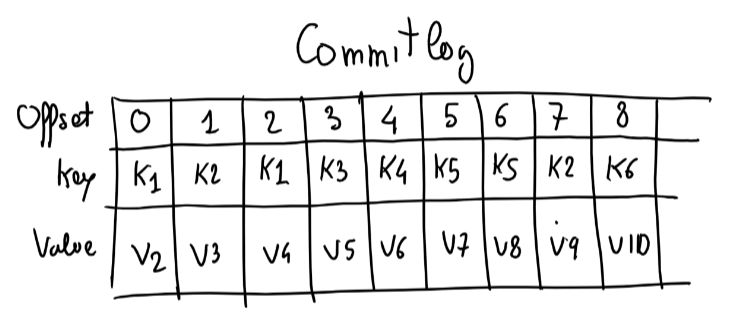
\includegraphics[width=0.6\textwidth]{figures/commit_log.png}
        \label{fig:commit_log}
        \caption{Commit log}
    \end{figure}

    \item A consumer reads messages from a topic. The consumer specifies the topic and the partition to 
    read from. The consumer reads messages in order of their offset, starting from the last offset read.

\end{enumerate}

Note that each broker can configure its log retention policy, which determines how long messages are 
kept in the commit log. This allows Kafka to manage the storage of messages and prevent the log from
growing indefinitely. In general, the default retention policy is to keep messages for a certain amount
of time, after which they are deleted, but we can also configure the retention policy to be based on
the size of the log, or the number of messages in the log.\\

Also, when deleting a log, there is a concept of \textbf{compaction}, which is a process that removes
duplicate messages from the log. This is useful when we want to keep only the latest version of a message,
and discard older versions. Compaction is useful for maintaining the state of a system, and for ensuring
that the log does not grow too large.\\

When making replicas, Kafka uses a leader-follower model. Each partition has one leader and multiple 
followers (replicas). The leader is responsible for handling reads and writes, while the followers are
responsible for replicating the data. If the leader fails, one of the followers is elected as the new 
leader, and the system continues to operate.

\subsection{Distributed consumption}

Kafka allows for distributed consumption, which means that multiple consumers can read messages from a
topic in parallel. This allows Kafka to scale out by distributing the load across multiple consumers.\\

Consumers can be part of a consumer group, which is a group of consumers that work together to read
messages from a topic. Each consumer in the group reads messages from a different partition, so that
the load is distributed evenly across the consumers. If a consumer fails, then the partitions that it
was reading from are reassigned to other consumers in the group, so that the system continues to operate.

\begin{figure}[H]
    \centering
    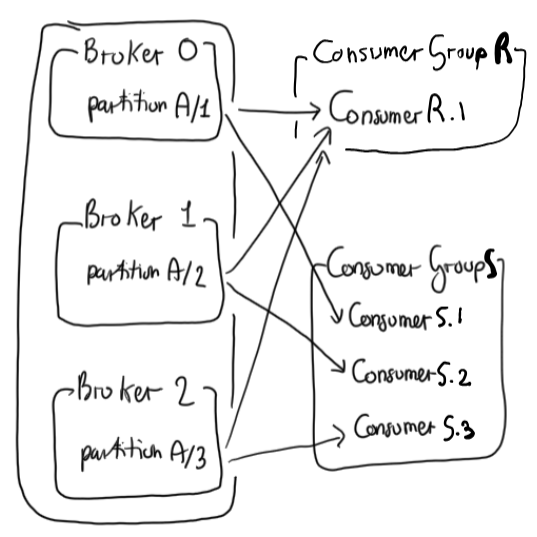
\includegraphics[width=0.4\textwidth]{figures/consumer_group.png}
    \label{fig:consumer_group}
    \caption{Consumer group}
\end{figure}

In general, Kafka provides at-least-once delivery guarantees, which means that messages are delivered
to consumers at least once. This is because Kafka stores messages in the commit log, and consumers can
re-read messages if needed. However, Kafka does not provide exactly-once delivery guarantees,
which means that messages can be delivered more than once.

\section{Apache Spark}

Apache Spark is an unified analytics engine for big data processing, with built-in modules for
streaming, SQL, machine learning, and graph processing. It is designed to be fast, easy to use, and
general-purpose. Spark is used by many companies, including Netflix, Uber, and Airbnb, to process
data at scale.\\

Spark is built around the concept of Resilient Distributed Datasets (RDDs), which are fault-tolerant
collections of objects that can be operated on in parallel. RDDs are the fundamental data structure
in Spark, and are used to represent data that is distributed across a cluster of machines.

\subsection{Key concepts in Spark}

Let us discuss some key concepts in Spark:

\begin{itemize}
    \item \textbf{Use RAM instead of disk}: Spark is designed to use RAM instead of disk for storing
    intermediate results. This allows Spark to be much faster than traditional MapReduce systems, which
    use disk for storing intermediate results.

    \begin{figure}[H]
        \centering
        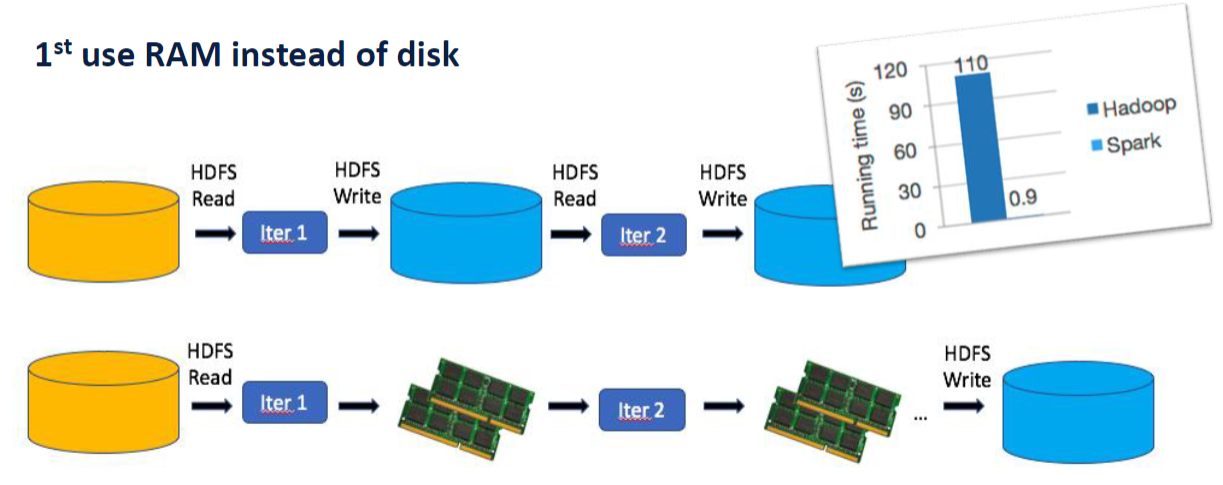
\includegraphics[width=0.6\textwidth]{figures/use_RAM.png}
        \label{fig:spark_ram}
        \caption{Spark in-memory processing}
    \end{figure}

    \item \textbf{Ease of use}: Spark provides a high-level API that makes it easy to write distributed
    programs. The API is available in multiple languages, including Scala, Java, Python, and R.

    \item \textbf{Generality}: Spark is a general-purpose computing engine that can be used for a wide
    range of applications, including batch processing, real-time processing, machine learning, and graph
    processing. This makes Spark a versatile tool that can be used for many different use cases.

    \begin{figure}[H]
        \centering
        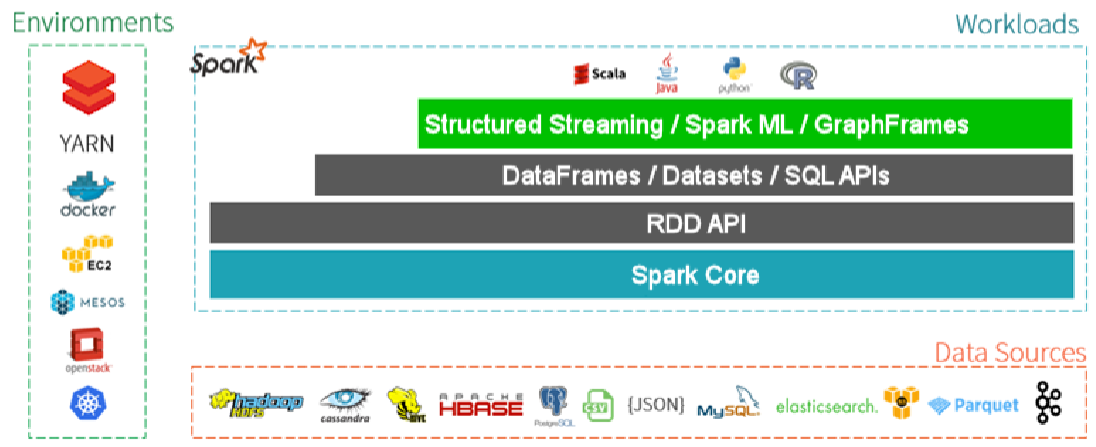
\includegraphics[width=0.6\textwidth]{figures/spark_generality.png}
        \label{fig:spark_generality}
        \caption{Spark generality}
    \end{figure}

\end{itemize}


\subsection{Resilient Distributed Datasets (RDDs)}

RDDs are the fundamental data structure in Spark. They are fault-tolerant collections of objects that
can be operated on in parallel. RDDs are immutable, which means that they cannot be changed once they
are created. Instead, transformations are applied to RDDs to create new RDDs.\\

RDDs can be created from a variety of data sources, including HDFS, S3, Cassandra, and Kafka. Once
created, RDDs can be transformed using a variety of operations, including map, filter, reduce, and join.
These operations are applied in parallel across the cluster, so that the processing is distributed
across multiple machines.

\subsubsection{Transformations and actions}

In Spark, there are two types of operations that can be applied to RDDs: transformations and actions.
Transformations are operations that create a new RDD from an existing RDD, while actions are operations
that return a value to the driver program.\\

Some common transformations in Spark include:

\begin{itemize}
    \item \textbf{map}: Applies a function to each element in the RDD.
    \item \textbf{filter}: Filters the elements in the RDD based on a predicate.
    \item \textbf{reduce}: Aggregates the elements in the RDD using a commutative and associative function.
    \item \textbf{join}: Joins two RDDs based on a key.
\end{itemize}

Some common actions in Spark include:

\begin{itemize}
    \item \textbf{collect}: Returns all the elements in the RDD to the driver program.
    \item \textbf{count}: Returns the number of elements in the RDD.
    \item \textbf{take}: Returns the first n elements in the RDD.
    \item \textbf{saveAsTextFile}: Saves the RDD to a text file.
\end{itemize}

\subsection{Spark at work}

Let us see how Spark can be used to process data. A Spark cluster consists of a driver program and
multiple worker nodes. The driver program is responsible for coordinating the execution of the job,
while the worker nodes are responsible for executing the tasks.

\begin{figure}[H]
    \centering
    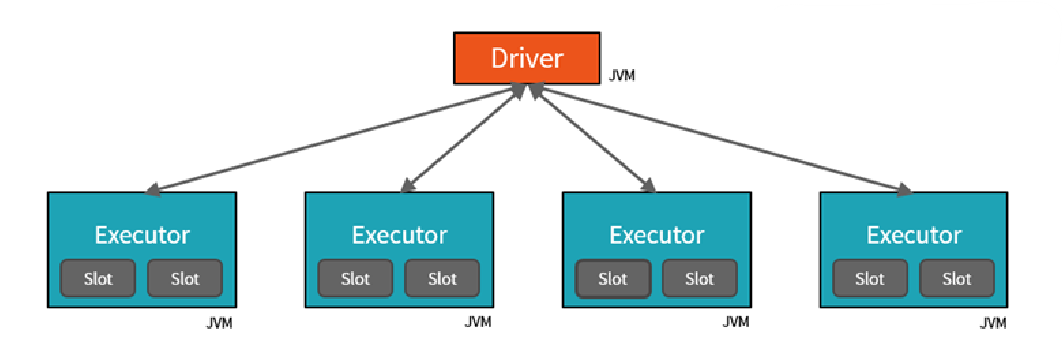
\includegraphics[width=0.7\textwidth]{figures/spark_components.png}
    \label{fig:spark_cluster}
    \caption{Spark components}
\end{figure}

When a job is submitted to the Spark cluster, the driver program breaks it down into stages, which are
then executed in parallel across the worker nodes. Each stage consists of tasks, which are executed
in parallel across the worker nodes. The tasks read data from RDDs, apply transformations to the data,
and write the results to new RDDs.

\begin{figure}[H]
    \centering
    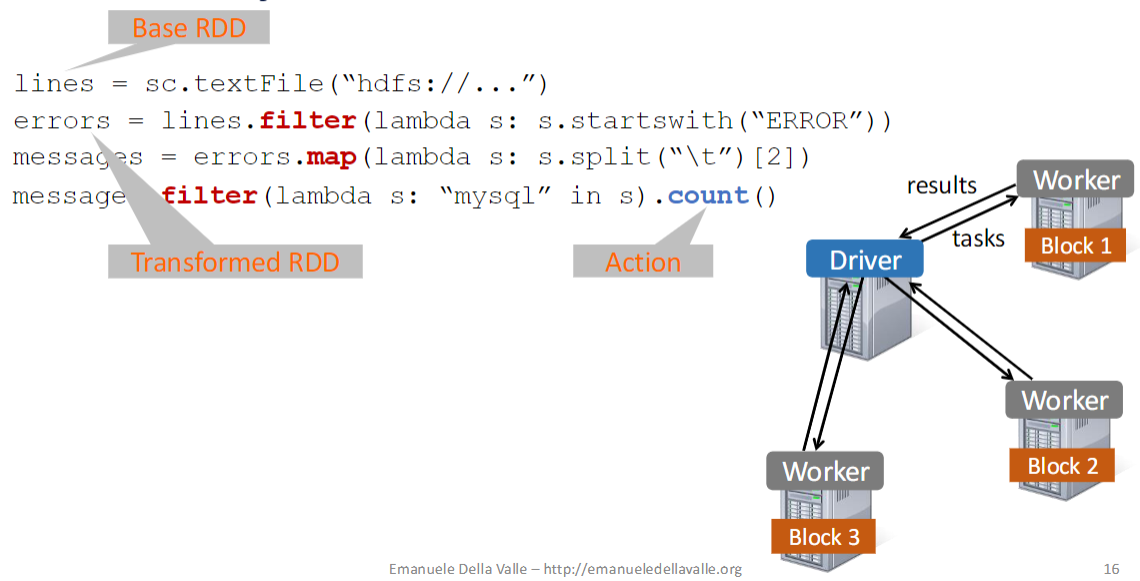
\includegraphics[width=0.7\textwidth]{figures/spark_execution.png}
    \label{fig:spark_execution}
    \caption{Spark execution model}
\end{figure}

In general, Spark uses a lazy evaluation model, which means that transformations are not executed
immediately. Instead, they are queued up and executed when an action is called. This allows Spark to
optimize the execution of the job, by combining multiple transformations into a single stage, and
reducing the number of shuffles that are needed.\\

Spark also provides fault-tolerance through lineage, which is a record of the transformations that
were applied to an RDD. If a partition of an RDD is lost, Spark can recompute it by replaying the
transformations that were applied to the RDD. This allows Spark to recover from failures and continue
processing the data.\\

Spark also provides caching, which allows RDDs to be stored in memory for faster access. This is useful
when an RDD is used multiple times in a job, as it avoids the need to recompute the RDD each time it
is used. Caching can be done at different levels, including memory only, disk only, and memory and disk.

\begin{figure}[H]
    \centering
    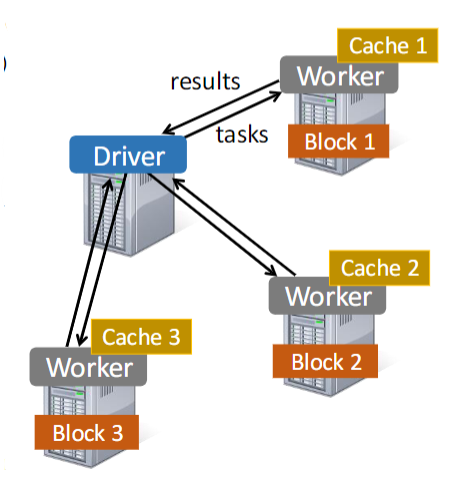
\includegraphics[width=0.35\textwidth]{figures/spark_caching.png}
    \label{fig:spark_caching}
    \caption{Spark caching}
\end{figure}

\subsection{DataFrames in Spark}

DataFrames are a high-level API for working with structured data in Spark. They provide a more
user-friendly interface than RDDs, and are optimized for performance. DataFrames are built on top
of RDDs, and provide a more structured way to work with data.\\

DataFrames can be created from a variety of data sources, including JSON, CSV, and Parquet files.
Once created, DataFrames can be queried using SQL, and transformed using a variety of operations,
including select, filter, groupBy, and join. These operations are optimized for performance, and
are executed in parallel across the cluster.\\

Let us see an example of how to create a DataFrame in Spark:

\begin{lstlisting}[language=Python]
from pyspark.sql import SparkSession

# Create a Spark session
spark = SparkSession.builder.appName("example").getOrCreate()

# Create a DataFrame from a JSON file
df = spark.read.json("data.json")

# Show the first 5 rows of the DataFrame
df.show(5)

# Filter the DataFrame
filtered_df = df.filter(col("age") > 30)

# Create a temporary view to query the DataFrame using SQL
filtered_df.createOrReplaceTempView("filtered_df")

# Query the DataFrame using SQL
query = "SELECT * FROM filtered_df"
result = spark.sql(query)
\end{lstlisting}

\subsubsection{Catalyst and Tungsten}

DataFrames in Spark are built on top of two key components: Catalyst and Tungsten. Catalyst is a query
optimizer that optimizes the execution of DataFrame operations. It uses a rule-based optimizer to
transform the query plan and generate an optimized plan. Tungsten is a memory-centric execution engine
that optimizes the execution of DataFrame operations. It uses code generation and memory management
techniques to improve the performance of the operations.\\

Together, Catalyst and Tungsten provide a high-performance engine for working with structured data in
Spark. They optimize the execution of DataFrame operations, and provide a more user-friendly interface
for working with data.

\section{Spark Structured Streaming}

Spark Structured Streaming provides a fast, scalable, fault-tolerant, end-to-end exactly-once stream
processing engine, without the user having to reason about streaming. It is built on the Spark SQL
engine, and provides a high-level API for working with streaming data. Structured Streaming allows
users to write streaming queries in the same way as batch queries, and provides the same fault-tolerance
and exactly-once guarantees as batch processing.

\subsection{Programming model}

Spark Structured Streaming treats a live data stream as an unbounded table, which is continuously
updated as new data arrives. As a result of this idea, users can logically express streaming computation
as a Directed Acyclic Graph (DAG) of standard batch-like queries on static tables. Spark will physically
run this DAG incrementally and continuously on the streaming data.\\

It uses the model of a DSMS (Data Stream Management System), as we saw in previous chapters. In every 
micro-batch, Spark will execute the DAG incrementally to update the final result. For each query, it will
mantain a state, which is updated in each micro-batch. We can see this in the following figure:

\begin{figure}[H]
    \centering
    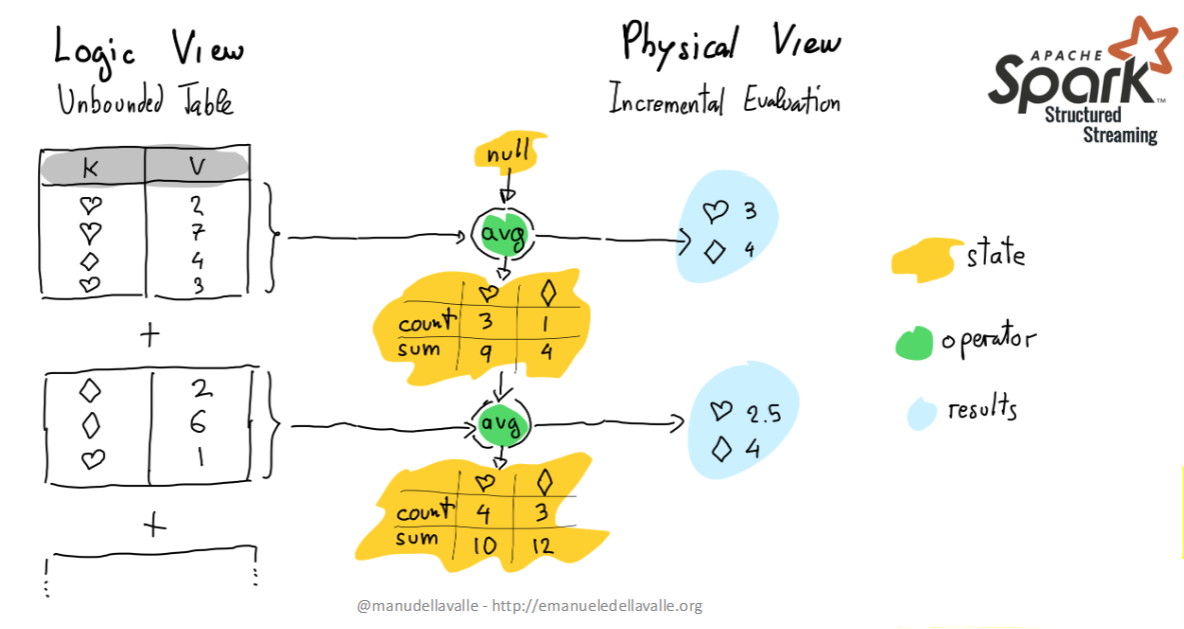
\includegraphics[width=0.7\textwidth]{figures/spark_increm_eval.png}
    \label{fig:spark_increm_eval}
    \caption{Spark incremental evaluation}
\end{figure}

It is important to note that Spark Structured Streaming does not materialize the entire table,
but only the incremental changes to the table. It will read the latest available data from the
stream, process it incrementally to update the result, and then discard the data. It will only
keep around the minimal intermediate state data as required to update the result, for example,
the intermediate counts and average for the above example.\\

This model is very powerful, as it allows users to express complex streaming computations in a
simple and declarative way, and provides the same fault-tolerance and exactly-once guarantees
as batch processing. It also allows users to easily integrate streaming and batch processing,
as the same code can be used for both.

\subsection{Creating streaming DataFrames}

To create a streaming DataFrame, we can use the \texttt{readStream} method of the SparkSession object.
It can receive as input the following sources:

\begin{itemize}
    \item File sources, i.e., a folder in which new files get dropped.

    \item Kafka sources, i.e., a Kafka topic.
    
    \item Socket sources, i.e., a TCP socket. This is only for testing purposes, as it does not
    provide fault-tolerance.
\end{itemize}

Let us see an example of how to create a streaming DataFrame in Spark, reading from a Kafka topic:

\begin{lstlisting}[language=Python]
from pyspark.sql import SparkSession

# Create a Spark session
spark = SparkSession.builder.appName("example").getOrCreate()

# Create a streaming DataFrame from a Kafka topic
raw_df = spark.readStream.format("kafka") \
    .option("kafka.bootstrap.servers", "localhost:9092") \
    .option("startingOffsets", "earliest") \
    .option("subscribe", "topic") \
    .load()

# Show the first 5 rows of the streaming DataFrame
raw_df.show(5)
\end{lstlisting}

In this example, we create a streaming DataFrame from a Kafka topic. We specify the Kafka bootstrap
servers, the starting offsets, and the topic to subscribe to. We then show the first 5 rows of the
streaming DataFrame.\\

Note that when extracting data from Kafka, our \texttt{raw\_df} DataFrame will have the following
schema:

\begin{itemize}
    \item \texttt{key}: The key of the message, as a binary blob.
    \item \texttt{value}: The value of the message, as a binary blob.
    \item \texttt{topic}: The topic of the message, as a string.
    \item \texttt{partition}: The partition of the message, as an integer.
    \item \texttt{offset}: The offset of the message, as an integer.
    \item \texttt{timestamp}: The timestamp of the message, as a timestamp.
    \item \texttt{timestampType}: The timestamp type of the message, as an integer.
\end{itemize}

Here, the column that contains the actual data is the \texttt{value} column. We can extract the data
from this column using the \texttt{select} method, as we will see in the following example:

\begin{lstlisting}[language=Python]
# Extract the data from the value column
casting = ("CAST(key AS STRING)", "CAST(value AS STRING)") 
data_df = raw_df.selectExpr(*casting)
\end{lstlisting}

In this example, we extract the data from the \texttt{key} and \texttt{value} columns, and cast them
to strings. This allows us to work with the data as strings, which is more convenient for processing. 
But the data of value will be a stringified JSON object, so we need to parse it to a DataFrame. 
We can do this as follows:

\begin{lstlisting}[language=Python]
from pyspark.sql.functions import from_json

# Parse the data from the value column
schema = "id STRING, name STRING, age INT"
parsed_df = data_df.select(from_json("value", schema).alias("data"))

# Obtain the final DataFrame
final_df = parsed_df.select("data.*")
\end{lstlisting}

In this example, we parse the data from the \texttt{value} column using the \texttt{from\_json} function,
and specify the schema of the data as a string. We then select the fields of the data, and obtain the
final DataFrame. This allows us to work with the data as a structured DataFrame, which is more convenient
for processing.

\subsection{Writing streaming DataFrames}

We have to remember that Spark is a lazy evaluation engine, so we need to call an action to start the
execution of the streaming DataFrame. The most common action to start the execution of a streaming
DataFrame is the \texttt{writeStream} method. This method allows us to write the streaming DataFrame
to a sink, which can be a file, a Kafka topic, or a console.\\

To do so, we need to specify the following options:

\begin{itemize}
    \item \textbf{Output sink}: The sink to write the data to.
    \item \textbf{Output mode}: The mode to use when writing the data, i.e., append, complete, or update.
    \item \textbf{Query name}: (Optional) Name of the query, which can be used to identify the query in the Spark UI.
    \item \textbf{Trigger interval}: (Optional) The interval at which to trigger the query, i.e., processing time or event time.
    \item \textbf{Checkpoint location}: (Optional) The location to store the checkpoint data, which is used to recover from failures.
\end{itemize}

We have 3 different output modes:

\begin{itemize}
    \item \textbf{Append}: Only the new rows added to the result table since the last trigger will be written to the sink.
    This is only supported for queries where rows added to the result table are never updated. For example,
    queries with only \texttt{select}, \texttt{where}, \texttt{map}, \texttt{filter}, \texttt{flatmap}, \texttt{join}, etc.
    \item \textbf{Complete}: The entire result table will be written to the sink after every trigger.
    This is dangerous, as it can cause the sink to grow indefinitely, and can lead to out-of-memory errors.
    It is only supported for aggregation queries.
    \item \textbf{Update}: Only the rows in the result table that were updated since the last trigger will be written to the sink.
    Supported for aggregation queries and few others, not for joins.
\end{itemize}


\subsection{Window operations on Event Time}

Spark Structured Streaming supports only logical windows on event time. It allows for declaring 
tumbling, hopping and session windows, and it treats windows as a particular grouping criteria.
For example, suppose we use the example of the fire alarms. We have:\\

\begin{lstlisting}[language=Python]
temperature_sdf.groupBy(window("TS", "1 minutes", "30 seconds"), "SENSOR")
\end{lstlisting}

This will group the data in 1-minute windows, with a 30-second slide, and by sensor. This will
create a new column with the window start and end times, and group the data by this column.\\

It is important to note that Spark Structured Streaming does not support physical windows on event time,
as it is a continuous processing engine. This means that it does not have the concept of windows in the
traditional sense, and does not have the notion of window boundaries. Instead, it treats windows as a
logical grouping criteria, and processes the data continuously as it arrives.

\subsection{Joins}

Spark Structured Streaming supports joins between two streaming DataFrames. The following table describes
the types of joins that are supported:

\begin{figure}[H]
    \centering
    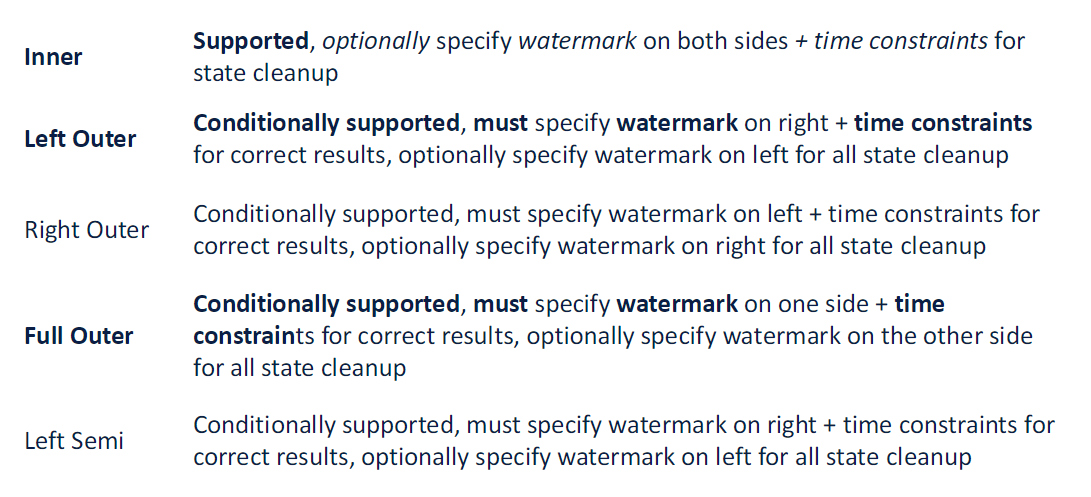
\includegraphics[width=0.75\textwidth]{figures/spark_joins.png}
    \label{fig:spark_joins}
    \caption{Spark joins}
\end{figure}

Note that, comparing Spark Structured Streaming with EPL, Spark does not support the "followed by"
operator (\texttt{->}). This is because Spark is a continuous processing engine, and does not have the
concept of events that are followed by other events. To achieve the same result, we need to use a 
stream-to-stream join with temporal constraints on the events timestamps. For example:\\

\begin{lstlisting}[language=Python]
join_sdf = smoke_events.join(
    high_temp_events, expr("""
        (sensorTemp == sensorSmoke) AND
        (tsTemp > tsSmoke) AND  ## this is the EPL's -> operator
        (tsTemp < tsSmoke + interval 2 minute)  ## this is the timer:within clause
    """)
)
\end{lstlisting}

Note that this will not tame the torrent effect, as it will report every event that matches the
condition, but this is expected. These two joins are equivalent:

\begin{lstlisting}[language=Python]
# Spark
join_sdf = A.join(B, expr("""
(idA == idB) AND
(tsB > tsA ) AND
(tsB < tsA + interval 2 minute )
"""))
\end{lstlisting}

\begin{lstlisting}[language=SQL]
# EPL
every x=A -> 
    every B(id=x.id)
    where timer:within(2 minutes)
\end{lstlisting}

Spark Structured Streaming also supports stream-to-table joins, which allow us to join a streaming
DataFrame with a static DataFrame. This is useful when we have a static lookup table that we want
to join with a streaming DataFrame. For example, suppose we have a static DataFrame with the sensor
information, and we want to join it with the streaming DataFrame with the temperature data. We can
do this as follows:

\begin{lstlisting}[language=Python]
# Create a static DataFrame with the sensor information
sensor_df = spark.read.csv("sensor.csv", header=True)

# Join the streaming DataFrame with the static DataFrame
join_sdf = temperature_sdf.join(sensor_df, "SENSOR")
\end{lstlisting}

\subsection{Late arrivals}

Late arrivals refer to events that arrive after the expected time window in which they were supposed
to be processed. This happens because in real-time streaming, data may experience delays due to 
temporarily disconnection, network high latency, processing issues, etc.\\

To handle late arrivals, Spark Structured Streaming provides a watermarking mechanism. Watermarking
allows us to specify a threshold on event time, after which we consider the data to be late. This
allows us to handle late arrivals by specifying a window on event time, and discarding data that
arrives after the window has closed.\\

To use watermarking, we need to specify the following options:

\begin{itemize}
    \item \textbf{Event time column}: The column that contains the event time.
    \item \textbf{Watermark delay}: The threshold on event time, after which we consider the data to be late.
\end{itemize}

The system will track the processing time $P$ as the maximum seen event time (last event time), and if
if the difference between $P$ and the event time of the event is smaller than the watermark delay, the
event is considered on time. Otherwise, it is considered late, and it is discarded.\\

To use watermarking, we need to specify the event time column and the watermark delay in the query.
For example, suppose we have a streaming DataFrame with the temperature data, and we want to handle
late arrivals. We can do this as follows:

\begin{lstlisting}[language=Python]
# Create a watermark column
watermarked_df = temperature_sdf.withWatermark("TS", "2 minutes")

# Group the data by window and sensor
windowed_df = watermarked_df.groupBy(window("TS", "1 minutes", "30 seconds"), "SENSOR")
\end{lstlisting}

In this example, we create a watermark column on the \texttt{TS} column with a delay of 2 minutes.
This allows us to handle late arrivals by specifying a window on event time, and discarding data that
arrives after the window has closed. We then group the data by window and sensor, and process the data
accordingly.\\

The following graph shows how watermarking works, in a windowed groped aggregation with update mode:

\begin{figure}[H]
    \centering
    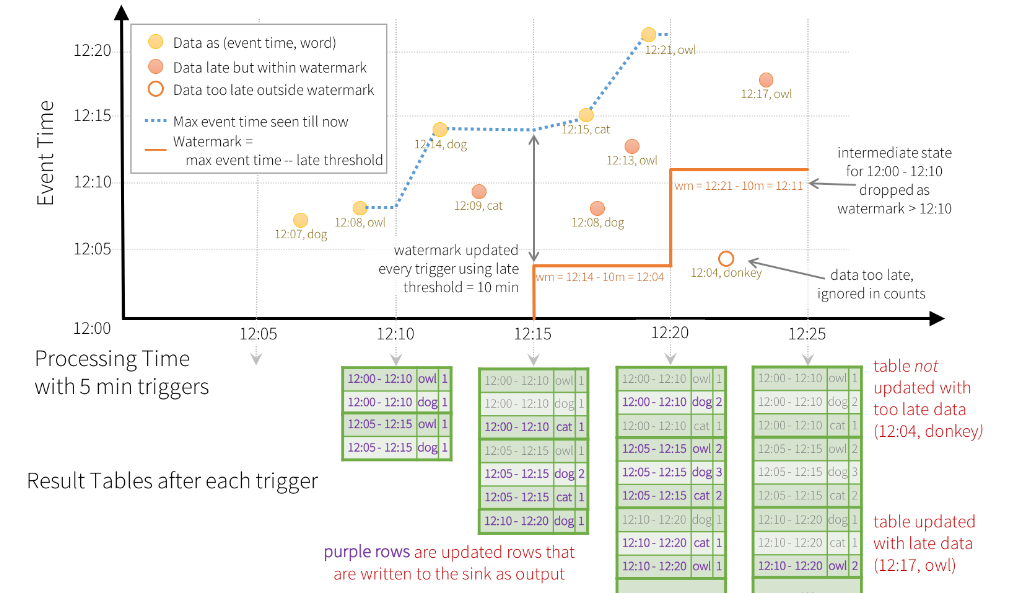
\includegraphics[width=0.9\textwidth]{figures/spark_watermark_update.png}
    \label{fig:spark_watermark_update}
    \caption{Spark watermarking in update mode}
\end{figure}

And the following graph shows how watermarking works, in a windowed groped aggregation with append mode:

\begin{figure}[H]
    \centering
    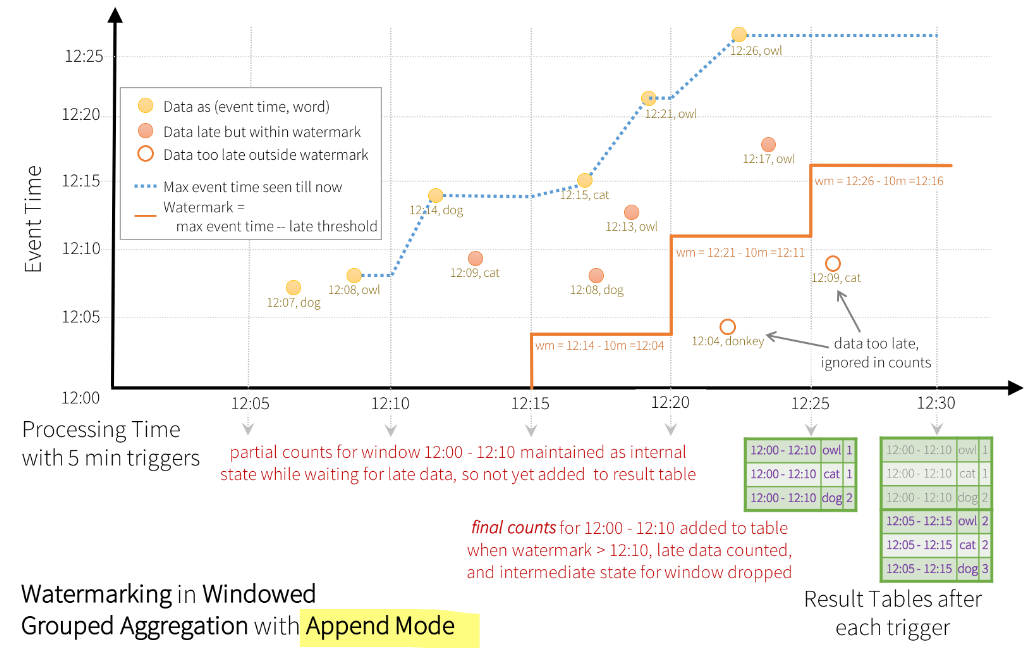
\includegraphics[width=0.9\textwidth]{figures/spark_watermark_append.png}
    \label{fig:spark_watermark_append}
    \caption{Spark watermarking in append mode}
\end{figure}

Note that a watermark delay of "X hours" guarantees that the engine will never
drop any data that is less than X hours late. However, data later that that
threshold is not guaranteed to be dropped. This data may or may not get aggregated,
and obviously the more delayed the data is, the less likely it is to be aggregated.

\subsection{Unsupported operations}

Spark Structured Streaming does not support all operations that are supported in batch processing.
Some of the operations that are not supported include:

\begin{itemize}
    \item Aggregation without grouping (e.g., counting rows of a table)
    \item OrderBy operations unless after aggregation and in Complete Output mode
    \item Limit and take the first N rows
    \item Distinct operations
    \item Chaining multiple stateful operations in Update and Complete mode
    \item Few types of outer joins
\end{itemize}